\documentclass[a4paper,leqno,9pt]{article}
\usepackage[utf8]{inputenc}
\usepackage{lmodern}
\usepackage{microtype}
\usepackage[inline]{enumitem}

\usepackage{siunitx}
\usepackage{multirow}
\usepackage{subcaption}

\usepackage[english]{babel}
\usepackage[autostyle, english=british]{csquotes}
\MakeOuterQuote{"}

\usepackage{commath}
\usepackage{amsmath}
\usepackage{amsthm}
\usepackage{amssymb}
\usepackage{mathtools}

\usepackage{pgfplots}
\pgfplotsset{compat=1.11}
\usepgfplotslibrary{fillbetween}
\usetikzlibrary{patterns}
\usetikzlibrary{arrows}

\usepackage{hyperref}

\usepackage[margin=1in]{geometry}
\usepackage{changepage}
\usepackage{titlesec}
\titleformat{\section}{\normalfont\Large\bfseries\centering}{Section~\thesection:}{1em}{}

\def\signed #1{{\leavevmode\unskip\nobreak\hfil\penalty50\hskip2em
  \hbox{}\nobreak\hfil(#1)%
  \parfillskip=0pt \finalhyphendemerits=0 \endgraf}}
\newsavebox\mybox
\newenvironment{aquote}[1]
  {\savebox\mybox{#1}\begin{quote}}
  {\signed{\usebox\mybox}\end{quote}}

% Augmented matrices.
\makeatletter
\renewcommand*\env@matrix[1][*\c@MaxMatrixCols c]{%
  \hskip -\arraycolsep
  \let\@ifnextchar\new@ifnextchar
  \array{#1}}
\makeatother

%--------grstep
% For denoting a Gauss' reduction step.
% Use as: \grstep{\rho_1+\rho_3} or \grstep[2\rho_5 \\ 3\rho_6]{\rho_1+\rho_3}
\newcommand{\grstep}[2][\relax]{%
   \ensuremath{\mathrel{
       {\mathop{\longrightarrow}\limits^{#2\mathstrut}_{
                                     \begin{subarray}{l} #1 \end{subarray}}}}}}
\newcommand{\swap}{\leftrightarrow}

\newtheoremstyle{exercise}% name of the style to be used
{5pt}% measure of space to leave above the theorem. E.g.: 3pt
{3pt}% measure of space to leave below the theorem. E.g.: 3pt
{\rm}% name of font to use in the body of the theorem
{}% measure of space to indent
{\large\bf}% name of head font
{.}% punctuation between head and body
{\newline}% space after theorem head; " " = normal interword space
{\thmname{#1}\thmnumber{ #2}\thmnote{: #3}}

\theoremstyle{exercise}
\newtheorem{exercise}{Exercise}

\theoremstyle{plain}
\newtheorem*{thm}{Theorem}
\theoremstyle{definition}
\newtheorem*{defn}{Definition}

\newcommand{\df}[1]{\textbf{#1}}
\newcommand{\T}{\mathrm{T}}
\newcommand{\F}{\mathrm{F}}
\newcommand{\IndSet}{\mathbf{I}}
\DeclareMathOperator{\cis}{cis}
\DeclareMathOperator{\arcsec}{arcsec}

\title{Level Three Conic Sections}
\author{Alex Elzenaar}
\date{\today}

\begin{document}
\setcounter{tocdepth}{1}

\begin{titlepage}
  \maketitle
  \begin{center}
    
\includegraphics[width=0.4\textwidth]{icecream}

    \vspace{2em}

    \begin{minipage}{\dimexpr\textwidth-4cm}
      \begin{aquote}{Menaechmus}\slshape
        O King, for traveling over the country, there are royal roads and roads for common citizens, but in geometry there is one road for all.
      \end{aquote}
    \end{minipage}
  \end{center}
  \thispagestyle{empty}
\end{titlepage}
\pagenumbering{arabic}

\tableofcontents
\section*{Preface}
The conic sections are the simplest curves in the plane which are not simply straight lines. However, most secondary school treatments of the subject
tend to present a set of vaguely connected case-by-case results, rather than any kind of coherent story. These notes are my attempt to avoid this.

Most of the content is presented as a series of exercises; however, even an enthusiastic Y13 student will require a significant amount of
guidance. As always, though, it is important that the student struggles with the material on their own!

\subsection*{Prerequisites}
These notes have perhaps the most `formal' prerequisites out of all my Y13 notes. I will assume results from trigonometry, linear systems, calculus, and
even algebra. However, this does not mean that the full power of these subjects are used. The most important prerequisites are actually Y11 and Y12
geometry because there are a number of results from there about triangles, circles, lines, and so forth that will be used here. My Y13 notes on trigonometry
revise a number of these results, and so the reader is directed there initially.

\begin{center}
  
\includegraphics[width=0.5\textwidth]{conics}
\end{center}

\titleformat{\section}{\clearpage\titlerule[0.8pt]\vspace{0.5ex}\normalfont\Large\bfseries\centering}{Section~\thesection:}{1em}{}[{\titlerule[0.8pt]}]
\let\oldsection\section
\renewcommand\section{\clearpage\oldsection}
\section{Introduction}
The study of the conic sections (as with much of elementary plane and solid geometry) goes back to the ancient Greeks. It is
thought that the first prson to study the slices of a cone was Menaechmus, who lived on the Gallipoli Peninsula in around 350~BCE,
in his solution of the Delian problem: the construction of a cube whose volume is twice that of a given cube. Anecdotally, it is to
Menaechmus that the famous quote on the cover of these notes is attributed (usually in his disputed role as the tutor to Alexander the Great).

Euclid of Alexandria published his book \emph{Elements}, one of the most influential mathematical texts of all time, in around
300~BCE (for perspective, this is around thirty years after the death of Alexander the Great). In it, he set down the set
of basic results which can be proved true about circles and lines on a plane: while modern geometry has gone much further than
Euclid (in considering geometry in more than two dimensions, and on surfaces much more complicated than the plane), the basic
results which are taught in any introductory geometry course are usually treated in the Elements.

As well as studying circles and lines, Euclid wrote a treatise on the conic sections. Unfortunately, it no longer survives;
however, Apollonius of Perga (a city in what is now Turkey) expanded Euclid's work and published his \emph{Conics} the century
after Euclid's death. Apollonius used Euclidean geometry to prove most of the classical theorems on the conic sections, including
the many applications to physics that the subject holds.

Conic sections have many beautiful applications; later on, we will discuss applications to optics and to celestial mechanics. For
example, in the 17th century the German astronomer Johannes Kepler showed that all astronomical bodies follow, due to gravity,
paths in the shape of conic sections.

This subject is also a very nice gateway into various topics in further mathematics, both in geometry and in analysis (calculus).

\section{Basic results}
\begin{defn}
  Let $ O $ be a fixed point and $ \ell $ be some line not passing through $ O $. A \df{conic} $ \mathcal{C} $ is the locus of a point $ P $ such
  that, if $ K $ is the point on $ \ell $ so that $ \ell \perp PK $,
  \begin{displaymath}
    \varepsilon = \frac{\abs{OP}}{\abs{PK}}
  \end{displaymath}
  where $ \varepsilon $ is some fixed constant.

  The point $ O $ is called the \df{focus}, the line $ \ell $ the \df{directrix}, and the constant $\varepsilon$ the \df{eccentricity}.
  The \df{latus rectum} (Latin: straight side) is defined to be the chord of a conic through the focus and parallel to the
  directrix; let $ l $ be the length of the latus rectum.

  The conic is variously called:
  \begin{itemize}
    \item an \df{ellipse} if $ \varepsilon < 1 $;
    \item a \df{parabola} if $ \varepsilon = 1 $; and
    \item an \df{hyperbola} if $ \varepsilon > 1 $.
  \end{itemize}

  \begin{center}
    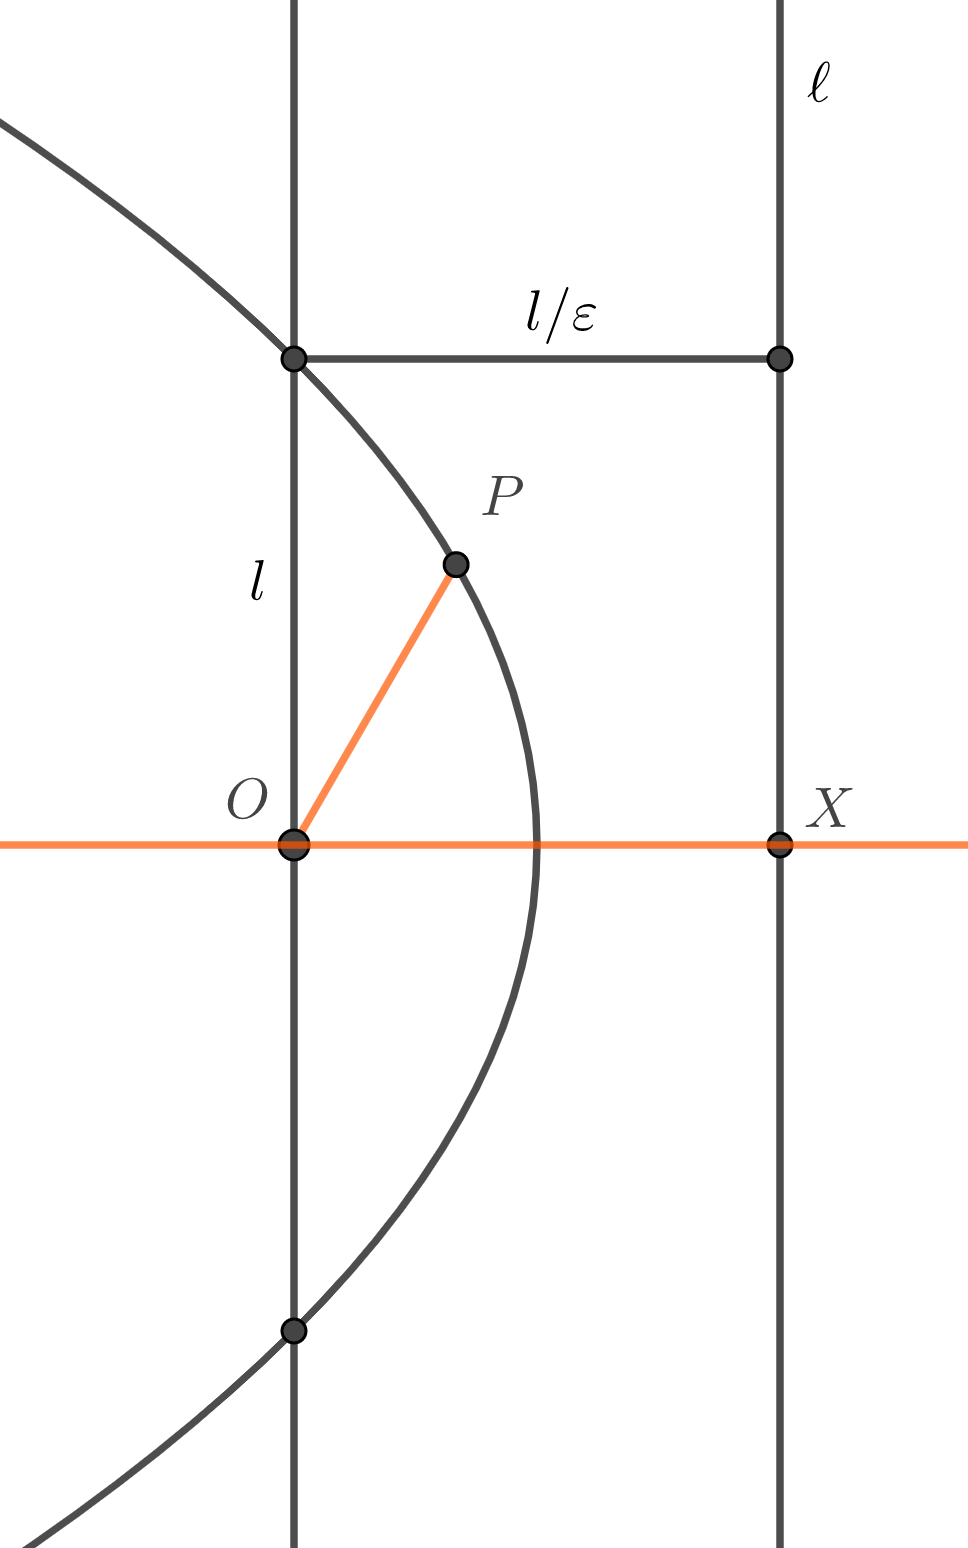
\includegraphics[width=0.3\textwidth]{polar}
  \end{center}
\end{defn}

\begin{exercise}[Polar form]
  Show that, if $ X $ is on the directrix of a conic such that $ OX \perp \ell $, then the polar equation of the
  conic with respect to this axis and origin $ O $ is
  \begin{displaymath}
    \frac{l}{r} = 1 + \varepsilon \cos \theta.
  \end{displaymath}
  Conclude that:
  \begin{enumerate}
    \item Every conic is symmetric with respect to $ OX $.
    \item The ellipse is a closed and bounded curve (i.e. it does not extend towards infinity).
    \item The parabola is unbounded, but is connected.
    \item The hyperbola consists of two seperate branches, each extending to infinity, given by $ -\alpha < \theta < \alpha $
          and $ \alpha < \theta < 2\pi - \alpha $ (where $ \alpha = \arcsec(-\varepsilon) $).
  \end{enumerate}
\end{exercise}

\begin{exercise}[Rectangular form]
  By squaring the polar form equation, show that the Cartesian equation for a conic, taking suitable axes and origin, is
  \begin{displaymath}
    x^2 + y^2 = (l - \varepsilon x)^2.
  \end{displaymath}
  \begin{enumerate}
    \item If $ \varepsilon \neq 1 $, and a suitable origin is chosen, show that the conic equation can be written in the form
          \begin{displaymath}
            \frac{x^2}{a^2} \pm \frac{y^2}{b^2} = 1
          \end{displaymath}
          for some real numbers $ a $ and $ b $. The new location of the origin is called the \df{centre} of the conic. Conclude that:
          \begin{enumerate}
            \item Both the ellipse and hyperbola are symmetric across both Cartesian axes.
            \item For an ellipse, the values $ 2a $ and $ 2b $ are the lengths of the chords through the origin along the $ x$- and $ y$-axes respectively.
            \item The two branches of a hyperbola lie in opposite regions formed by the two lines (\df{asymptotes})
                    \begin{displaymath}
                      \left(\frac{x}{a} - \frac{y}{b} \right)\left(\frac{x}{a} + \frac{y}{b} \right) = 0.
                    \end{displaymath}
                    The value $ 2a $ is the length of the transverse axis of the hyperbola and the value $ 2b $ is the length of the conjugate
                    axis: the two dimensions of the rectangle whose diagonals are the asymptotes and which is bounded by the hyperbola.
          \end{enumerate}
    \item If $ \varepsilon = 1 $, show that the conic equation for the parabola can be written in the form
          \begin{displaymath}
            y^2 = 2l(\frac{1}{2}l - x).
          \end{displaymath}
          By reflecting in a suitable vertical line, derive the standard form equation
          \begin{displaymath}
            y^2 = 2lx.
          \end{displaymath}
          Given this latter equation, give the coordinates of the focus, and the Cartesian equation of the directrix.
  \end{enumerate}
\end{exercise}

\begin{exercise}[Parametric form]
  Show that:
  \begin{enumerate}
    \item The ellipse $ x^2/a^2 + y^2/b^2 = 1 $ is parameterised by $ (a \cos t, b \sin t) $ for $ 0 \leq t < 2\pi $.
    \item The parabola $ y^2 = 2lx $ is parameterised by $ (2lt^2, 2lt) $.
    \item The hyperbola $ x^2/a^2 - y^2/b^2 = 1 $ is parameterised by $ (a \sec t, b \tan t) $ for $ 0 \leq t < 2\pi $.
  \end{enumerate}
  Illustrate these parameterisations with a suitable computer program (e.g. Geogebra, or your favourite programming language).
\end{exercise}

\begin{exercise}[Focii of rectangular conics]
  Given the equation
  \begin{displaymath}
    \frac{x^2}{a^2} \pm \frac{y^2}{b^2} = 1,
  \end{displaymath}
  compute the coordinates of the focus, equation of the directrix, and eccentricity of the conic. Hence show that
  ellipses and hyperbolae have two focii and two directrices each. Where is the directrix of a circle?

  Show that the following two properties can be used as alternative definitions for the ellipse and hyperbola:
  \begin{enumerate}[label={AP\arabic*}.]
    \item Show that the ellipse with focii $ O_1 $ and $ O_2 $ is the locus of all points $ P $
          such that $ d(O_1, P) + d(P, O_2) = R $ for some constant $ R $. Give $ R $ in terms of $ a $ and $ b $.
    \item Show that the hyperbola with focii $ O_1 $ and $ O_2 $ is the locus of all points $ P $
          such that $ d(O_1, P) - d(P, O_2) = R $ for some constant $ R $. Give $ R $ in terms of $ a $ and $ b $.
  \end{enumerate}

  As an application of this definition, we will derive the `reflection property' of the ellipse.
  \begin{enumerate}
    \item Suppose $ O_1 $ and $ O_2 $ are on the same side of a line $ \ell $. Show that the shortest path from $ O_1 $
          to $ O_2 $ which touches the line $ \ell $ is the broken line $ O_1XO_2 $, where $ X $ is on $ \ell $ and
          the angles between $ O_1 X $ and $ \ell $ and between $ X O_2 $ and $ \ell $ are equal. (Hint: you can do this
          with calculus, but that would be like killing a fly with a sledgehammer.)
    \item Show that, if $ O_1 $ and $ O_2 $ are two focii of an ellipse and $ X $ is any point on the ellipse, then the broken line $ O_1 X O_2 $
          makes equal angles with the tangent line of the ellipse at $ X $. (Hint: show that this broken line is the shortest path from $ O_1 $ to $ O_2 $
          that touches the tangent line at $ X $.)
    \item Thus, given the law of reflection for waves, show that if a light source is placed at $ O_1 $ then every ray from the source
          will arrive at $ O_2 $ at precisely the same time.
    \item Derive some result of this kind for parabolae by treating a parabola as an ellipse with one focus `at infinity'. Suggest an
          application of this property related to, say, torches.
  \end{enumerate}
\end{exercise}

\section{Isometries}
In the previous section, we saw geometrically that every ellipse or hyperbola is just a translated and rotated version of the graph of
an equation with the form
\begin{equation}
  \frac{x^2}{a^2} + \frac{y^2}{b^2} = 1.
\end{equation}
(Herein, in this section we will write $ p = 1/a^2 $ and $ q = 1/b^2 $ for convenience.)

Here, we will show this relation using coordinates --- the advantage of this approach is that it allows us to calculate precisely
from the equation of a conic its position and angle with respect to the standard axes. The subtle point here is basically that the
same curve will have different equations depending on its position in the coordinate system --- in the previous section we chose our
coordinate system in the `nicest way possible' by geometric means, and now we are given a conic already sitting in some coordinate
system which we want to understand.

In order to pursue this programme, we need to study the effect of rotations and translations on coordinate systems. We
begin with rotations because it turns out that rotating before translating is easier for our purposes.

Let $ \rho = \cis \theta $ be a complex number such that $ \abs{\rho} = 1 $. If $ z = x + yi $ is a point on the complex plane,
then $ \rho $ acts by multiplication on $ z $ to rotate it around the origin by an angle $ \theta $; we can then calculate
the resulting rectangular coordinates of $ \rho z $ to see how a rotation affects our normal coordinate system.
\begin{align*}
  z &= \abs{z} \cis(\tan^{-1} x/y)\\
  \rho z &= \abs{z} \cis(\tan^{-1} x/y + \theta)\\
         &= \abs{z} \left[\cos(\tan^{-1} x/y + \theta) + i\sin(\tan^{-1} x/y + \theta)\right].
\end{align*}

Using trig identities, we calculate
\begin{align*}
  \cos(\tan^{-1} x/y + \theta) = \cos(\tan^{-1} x/y) \cos \theta - \sin(\tan^{-1} x/y) \sin \theta\\
                               = \frac{x}{\sqrt{x^2 + y^2}} \cos \theta - \frac{y}{\sqrt{x^2 + y^2}} \sin \theta\\
  \sin(\tan^{-1} x/y + \theta) = \sin(\tan^{-1} x/y) \cos \theta + \cos(\tan^{-1} x/y) \sin \theta\\
                               = \frac{y}{\sqrt{x^2 + y^2}} \cos \theta + \frac{x}{\sqrt{x^2 + y^2}} \sin \theta
\end{align*}
and so
\begin{align*}
  \rho z &= \abs{z} \left[\cos(\tan^{-1} x/y + \theta) + i\sin(\tan^{-1} x/y + \theta)\right]\\
         &= (x \cos \theta - y \sin \theta) + i(y \cos \theta + x \sin \theta).
\end{align*}

In other words, if the point $ (x,y) $ is rotated about the origin by an angle $ \theta $, then
\begin{equation}
  (x,y) \xmapsto{\rho} (x \cos \theta - y \sin \theta,y \cos \theta + x \sin \theta).
\end{equation}

Considering $ ax^2 + bx + cxy + dy + ey^2 $, then, we want to rotate $ (x,y) $ by some $ \theta $ so that some terms vanish. Doing
a long computation, we find that
\begin{align*}
  ax^2 + bx + cxy + dx + ey^2 &\mapsto a(x \cos \theta - y \sin \theta)^2 + b(x \cos \theta - y \sin \theta)\\
                              &  \qquad + c(x \cos \theta - y \sin \theta)(y \cos \theta + x \sin \theta)\\
                              &  \qquad + d(y \cos \theta + x \sin \theta) + e(y \cos \theta + x \sin \theta)^2\\
                              &= x^2(a\cos^2 \theta + \frac{c}{2}\sin 2\theta + e\sin^2 \theta) + x(b \cos \theta + d\sin \theta)\\
                              &  \qquad + xy ((e - a)\sin 2\theta + c \cos 2\theta)\\
                              &  \qquad + y(-b \sin \theta + d \cos \theta) + y^2(a\sin^2 \theta - \frac{c}{2}\sin 2\theta + e\cos^2 \theta)
\end{align*}
and, looking at this, we see that an easy candidate we can try to get rid of is the $ xy $ term. In fact, if we want this term
to be zero we need only solve
\begin{equation}
  (e - a)\sin 2\theta + c \cos 2\theta = 0
\end{equation}
which is easy: $ \frac{-c}{e - a} = \frac{\sin 2\theta}{\cos 2\theta} = \tan 2\theta $, and so in order to remove
the $ xy $ term we need only rotate our coordinate system by
\begin{equation}
  \theta = \frac{1}{2}\tan^{-1} \frac{c}{a - e}.
\end{equation}

Making the coordinate system change $ (x,y) \mapsto (x \cos \theta - y \sin \theta,y \cos \theta + x \sin \theta) $ therefore leaves
us with something that looks like $ ax^2 + bx + dy + ey^2 = 1 $, where $ x $ and $ y $ are now coordinates in our rotated coordinate
system and where the constants $ a $ to $ e $ are not necessarily the same as before.

We already know that if $ y = f(x) $ is graphed, then we can shift the graph up by $ x_0 $ and to the right
by $ y_0 $ by suitable transformations of the coordinates: $ y - y_0 = f(x - x_0) $ has the shifted graph. Last
year, we performed similar transformations on parabolae by completing the square, and so this is the technique
which we will use now. We proceed as we did last year (but now completing the square in both $ x $ and $ y $):
\begin{displaymath}
  ax^2 + bx + dy + ey^2 = a\left(x + \frac{b}{2a}\right)^2 - \frac{b^2}{4a} + e\left(\frac{d}{2e} + y\right)^2 - \frac{d^2}{4e} = 1.
\end{displaymath}
If we now let $ (x, y) \mapsto \left(x - \frac{b}{2a}, y - \frac{d}{2e}\right) $, then we have got a coordinate
transformation that removes all the linear terms and leaves us with something like
\begin{displaymath}
  ax^2 + ey^2 = 1 + \frac{b^2}{4a} + \frac{d^2}{4e}
\end{displaymath}
and upon division of both sides by $ 1 + \frac{b^2}{4a} + \frac{d^2}{4e} $ we end up, as promised, with something of
the form $ px^2 + qy^2 = 1 $. Note that our coordinate system has completely changed: the new curve has the same
shape as our original curve, but sits inside our new coordinate system much more naturally than it sat in our old
coordinate system.

\begin{exercise}[Further thoughts on this argument]\label{exercise:degenerate}
  You are asked to think critically about the above argument (so reread it and check the computations) and to extend it (so not only must
  you read it, but understand it).
  \begin{enumerate}
    \item Clearly $ y = x^2 $ cannot be written in the canonical form. Where does the proof above fall down for a parabola?
    \item What happens if our ellipse is a circle?
    \item We have now classified the quadratic equations in two variables corresponding to hyperbolae and ellipses ($ px^2 \pm qy^2 = 1 $)
          and parabolae ($ y^2 = kx^2 $). What other forms can the graph of such a quadratic equation take? (Hint: you should be able to
          find three other kinds, and show that every quadratic equation is of one of the six kinds.)
  \end{enumerate}
\end{exercise}

\begin{exercise}[Computations]
  First, read the following quote:

  \vspace{3pt}

  \hfill\begin{minipage}{\dimexpr\textwidth-1cm}
    The attitude adopted in this book is that while we expect to get numbers out of the machine, we also expect to take action based on them, and, therefore we need to understand thoroughly what numbers may, or may not, mean. To cite the author's favorite motto,

    ``The purpose of computing is insight, not numbers,'' although some people claim,

    ``The purpose of computing numbers is not yet in sight.''

    There is an innate risk in computing because ``to compute is to sample, and one then enters the domain of statistics with all its uncertainties.''
    \begin{flushright}
      --- Richard W. Hamming, \textit{Introduction to applied numerical analysis}, McGraw-Hill 1971, p.31. (Quoted in \url{https://mathoverflow.net/a/7164}.)
    \end{flushright}
  \xdef\tpd{\the\prevdepth}
  \end{minipage}

  \begin{enumerate}
    \item Classify the following conics:
          \begin{enumerate}
            \item $ \frac{10}{4}x^2 + 3xy + \frac{10}{4}y^2 = 1 $
            \item $ 4x^2 + 24xy + 11y^2 = 5 $
          \end{enumerate}
    \item What happens to the equation for the hyperbola $ x^2 - y^2 = a^2 $ upon rotation by $ \pi/4 $?
    \item Give an equation for the parabola with vertex $ (0,2) $, and with axis $ y = x + 2 $ (opening into the positive $ x$-half plane).
    \item Find the two focii of an ellipse passing through $ (0,0) $, $ (0, 1) $, and $ (1,2) $.
  \end{enumerate}
\end{exercise}

\section{Cones}
\begin{center}
  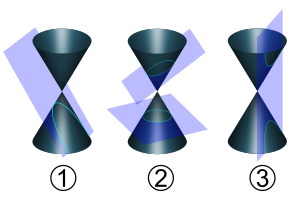
\includegraphics[width=0.5\textwidth]{slices}
\end{center}
We now move from the planar definitions of the conics to the `cone-slicing' definitions. Essentially, our goal
is to show that the conics are just slices of a cone (hence the name), as in the diagram above.\footnote{By Pbroks13 - Own work, CC BY 3.0, \url{https://commons.wikimedia.org/w/index.php?curid=5919064}}

\begin{exercise}[Defining a cone]
  We will define a cone to be the locus of all lines in three dimensional space which pass through the origin and through a point on some
  fixed curve in the plane $ z = 1 $. Note: to show a given object is a cone, one must guess a good defining curve (usually by intersecting
  it with the given plane) and then do two things: (N1) show that every line through the origin and a point on the guessed curve lies on the
  object, and (N2) show that every point on the object lies on such a line.
  \begin{enumerate}
    \item Give various non-examples of cones, especially surfaces satisfying critera N1 but not N2 and those satisfying N2 but not N1.
    \item Show that $ x^2 + y^2 = cz^2 $ is a cone whose defining curve is a circle; show that the line through the origin and the centre
          of this circle cuts the $ z = 1 $ plane at right angles. (This cone is called a \df{right circular cone}.)
    \item Show that $ ax^2 + by^2 + cz^2 = 0 $ is a cone for every value of $ a $, $ b $, and $ c $. What is its defining curve?
  \end{enumerate}
\end{exercise}

\begin{exercise}[Algebraic cone-slicing]
  Show that all six kinds of conic sections which you found in exercise \ref{exercise:degenerate} are indeed obtained by
  slicing cones with planes.

  \textit{Hints:}
  \begin{itemize}
    \item Fix a cone, say $ x^2 + y^2 = cz^2 $, and then slice it with various planes.
    \item The plane through $ (x_0, y_0, z_0) $ which is orthogonal to the line between $ (0,0,0) $ and $ (a,b,c) $ is given by
          \begin{displaymath}
            a(x-x_0) + b(y-y_0) + c(z-z_0) = 0.
          \end{displaymath}
          If you use this fact, you need not prove it.
  \end{itemize}
\end{exercise}

\begin{exercise}[Geometric cone-slicing: the icecream proof]
  In the previous exercise, we had to use coordinates to prove that every slice of a cone is a conic. We will now
  discover a geometric proof that an ellipse is just a slice of a right circular cone, in such a way that we will
  understand why such slices obey the focii properties of the ellipse.\footnote{~This proof is as given in Apostol, \textit{Linear~Algebra} ---
  the figure used is Figure 2.11 from that book --- but it is originally due to Dandelin.}

  Let us take our plane and slice our cone with it. Pick any point $ P $ in the intersection of the two surfaces (i.e.
  on the curve we wish to show is an ellipse). In addition, we will place two spheres $ S_1 $ and $ S_2 $ into our cone
  such that they are tangent to both the cone and to the plane. Let $ F_1 $ and $ F_2 $ be the two points of contact between
  the plane and the spheres, and let $ C_1 $ and $ C_2 $ be the circles of contact between the cone and the spheres.

  \begin{center}
    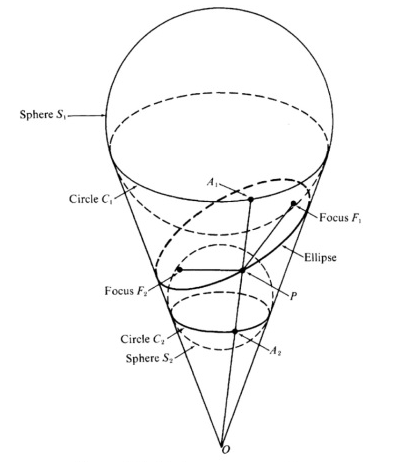
\includegraphics[width=0.5\textwidth]{apostol}
  \end{center}

  \begin{enumerate}
    \item Show that if $ X $ is a point outside some sphere, and if $ M $ and $ N $ are points on the sphere such that $ XM $
          and $ XN $ are tangent lines to the sphere, then $ \abs{XM} = \abs{XN} $. (Hint: consider the cross-section of the sphere
          obtained by slicing it with the plane of the triangle $ XMN $.)
    \item Suppose the vertex of our cone is $ O $. Show that if $ A_1 $ and $ A_2 $ are the points of intersection
          between the line $ OP $ and the two circles $ C_1 $ and $ C_2 $ then $ \abs{PF_1} = \abs{PA_1} $ and $ \abs{PF_2} = \abs{PA_2} $.
    \item Show that $ \abs{PA_1} + \abs{PA_2} $ is independent of the point $ P $.
    \item Conclude that $ \abs{PF_1} + \abs{PF_2} $ is constant for every value of $ P $, and therefore that the locus of $ P $
          is an ellipse with focii $ F_1 $ and $ F_2 $.
  \end{enumerate}
\end{exercise}

\section{Applications to physics}

\section{Further reading}
Kendig
Coxeter
Salmon

\end{document}
